\chapter{الأمواج الكهرمغناطيسية المستوية والاستقطاب}\label{ch:b2:plane-waves-polarization}

أمِل رأسك وأنت ترتدي نظارة شمسية مستقطِبة فيظهر وهج الطريق
المبتلّة ويختفي؛ وأدر النظارة أمام شاشة هاتف
فتسودّ الشاشة. فالضوء الذي يبلغ عينك ليس
موجةً ذات تواتر وشدة فحسب: بل له \emph{جهة
اهتزاز}، ويلعب بها كل مستقطِب وشاشة وعدسة سينما ثلاثية الأبعاد وواصل
ألياف بصرية. وهذا الفصل يحلّ \omterm{thm:b2:maxwell-equations:maxwell}{معادلات ماكسويل}
في الفضاء الخالي --- أي الموجة المستوية، بمجاليها الكهربائي
والمغناطيسي المستعرضين المقفلين متعامدين --- ويستعرض الطيف الذي
تمتد عليه تلك الأمواج، ويدرس الاستقطاب: كيف يوصف، وكيف
يُنتقى بمستقطِب (\omterm{prop:b2:plane-waves-polarization:malus}{قانون مالوس})، وكيف يُحوَّل بصفيحة
مضاعفة الانكسار.

\section{الأمواج المستوية في الخلاء}

\begin{theorem}[معادلة الأمواج؛ الأمواج المستوية المتقدمة التوافقية]\label{thm:b2:plane-waves-polarization:wave}
\index{موجة كهرمغناطيسية}\index{موجة مستوية (كهرمغناطيسية)}\index{استعراضية}
في الخلاء، الخالي من الشحن والتيارات، تعطي \omterm{thm:b2:maxwell-equations:maxwell}{معادلات ماكسويل}
\[
\Delta\vect E = \frac1{c^2}\frac{\partial^2\vect E}{\partial t^2} , \qquad
\Delta\vect B = \frac1{c^2}\frac{\partial^2\vect B}{\partial t^2} , \qquad
c = \frac1{\sqrt{\varepsilon_0\mu_0}} = \qty{2.998e8}{m/s} .
\]
و\emph{الموجة المستوية المتقدمة التوافقية} $\underline{\vect E} =
\underline{\vect E}_0\,\eu^{\iu(\omega t - \vect k\cdot\vect r)}$ حلّ شرط أن يكون
$\omega = ck$ (أي بلا تبدد)، وتقتضي \omterm{thm:b2:maxwell-equations:maxwell}{معادلات ماكسويل} عندئذ
\[
\vect k\cdot\vect E = 0 , \qquad
\vect B = \frac{\vect k\wedge\vect E}\omega = \frac{\vect u\wedge\vect E}c ,
\]
حيث $\vect u = \vect k/k$ جهة الانتشار: فالموجة
\emph{مستعرضة}، و $(\vect E, \vect B, \vect u)$ ثلاثي متعامد
مباشر، و $\vect E$ و $\vect B$ في طور واحد و $B = E/c$. وشدتها
$I = \varepsilon_0cE_0^2/2$ وتحمل تدفق كمية حركة $I/c$
(\cref{ch:b2:poynting-vector}).
\end{theorem}

\begin{proof}
اشتُقت \omterm{thm:b2:waves-on-strings:equation}{معادلة الأمواج} في \cref{exo:b2:maxwell-equations:11}.
ومن أجل $\eu^{\iu(\omega t - \vect k\cdot\vect r)}$، يصير $\partial_t \to \iu\omega$ و $\vect\nabla \to
-\iu\vect k$: ومنه $\Delta \to -k^2$، فيكون $k^2 = \omega^2/c^2$؛ ويعطي ماكسويل--غاوس $-\iu
\vect k\cdot\underline{\vect E} = 0$، وماكسويل--التدفق $\vect k\cdot\underline{\vect B} = 0$،
وماكسويل--فاراداي $-\iu\vect k\wedge\underline{\vect E} = -\iu\omega\underline{\vect B}$، ومنه
$\underline{\vect B} = \vect k\wedge\underline{\vect E}/\omega$، ومقياسها $kE/\omega = E/c$ وهي
عمودية عليهما؛ ثم يتحقق ماكسويل--أمبير تلقائيًّا.
\end{proof}

\begin{omfigure}
\begin{tikzpicture}[font=\small, x=1cm, y=1cm, >=Stealth]
  \draw[->, thick] (-0.3,0) -- (7.4,0) node[right, font=\footnotesize] {$\vect u$};
  \draw[omDef, thick, domain=0:6.8, samples=80] plot (\x,{1.1*cos(deg(1.2*\x))});
  \draw[omProp, thick, domain=0:6.8, samples=80] plot (\x,{-0.4*cos(deg(1.2*\x))});
  \foreach \x in {0,0.65,...,6.6} {
    \pgfmathsetmacro{\e}{1.1*cos(deg(1.2*\x))}
    \draw[omDef, ->] (\x,0) -- (\x,\e);
    \draw[omProp, ->] (\x,0) -- ({\x+0.55*\e*0.36},{-0.4*\e*0.9});
  }
  \node[omDef, font=\footnotesize] at (0.4,1.45) {$\vect E$}; \node[omProp, font=\footnotesize] at (0.9,-0.75) {$\vect B = \vect u\wedge\vect E/c$};
  \draw[<->] (0,-1.3) -- (5.24,-1.3) node[midway, below, font=\footnotesize] {$\lambda = 2\pi/k = c/f$};
\end{tikzpicture}

{\small موجة مستوية متقدمة توافقية في لحظة واحدة: $\vect E$ و
$\vect B$ عموديان أحدهما على الآخر وعلى جهة السير، وفي
طور واحد، و $B = E/c$؛ وينزلق النقش كله على امتداد $\vect u$ بالسرعة $c$.}
\end{omfigure}

\begin{remark}[الطيف]\label{rem:b2:plane-waves-polarization:spectrum}
\index{الطيف الكهرمغناطيسي}
معادلة واحدة وسرعة واحدة وعشرون رتبة قدر من التواتر.
الراديو: \qty{30}{kHz}--\qty{300}{MHz} ($\lambda$ من \qty{10}{km} إلى \qty{1}{m})،
والهوائيات والدارات (\cref{ch:b2:dipole-radiation}). والموجات الصغرية:
\qty{300}{MHz}--\qty{300}{GHz}، والرادار والأفران والهواتف المحمولة والخلفية
الكونية. وتحت الأحمر: حتى \qty{400}{THz} (أي \qty{750}{nm})، وهو الإشعاع
الحراري لكل ما حولنا (\cref{ch:b2:thermal-radiation}).
والمرئي: \qty{400}{THz}--\qty{750}{THz}، من \qty{750}{nm} (أحمر) إلى \qty{400}{nm}
(بنفسجي) --- أي ديوان واحد، وفوتونات من $1.6$ إلى \qty{3.1}{eV}. وفوق البنفسجي حتى
\qty{10}{nm}؛ والأشعة السينية حتى \qty{10}{pm} (أي \qty{100}{keV})، من الأغلفة الذرية الداخلية
ومن الإلكترونات المكبوحة؛ وأشعة غاما فيما وراء ذلك، من النوى. ولا تختلف إلا المنابع
والكواشف: أما الموجة فواحدة.
\end{remark}

\begin{omfigure}
\begin{tikzpicture}[font=\small, x=1cm, y=1cm, >=Stealth]
  \draw[->, thick] (0,0) -- (13.2,0) node[right, font=\footnotesize] {$f$};
  \foreach \x/\l in {0/$10^4$, 2/$10^6$, 4/$10^8$, 6/$10^{10}$, 8/$10^{12}$, 10/$10^{14}$, 12/$10^{16}$} {
    \draw (\x,-0.1) -- (\x,0.1); \node[font=\scriptsize, below] at (\x,-0.12) {\l};
  }
  \node[font=\scriptsize, below] at (13.0,-0.12) {Hz};
  \fill[omDef!30] (0,0.3) rectangle (4.5,1.0); \node[font=\footnotesize] at (2.25,0.65) {راديو};
  \fill[omDef!50] (4.5,0.3) rectangle (7.5,1.0); \node[font=\footnotesize] at (6.0,0.65) {موجات صغرية};
  \fill[omThm!30] (7.5,0.3) rectangle (10.6,1.0); \node[font=\footnotesize] at (9.05,0.65) {تحت الأحمر};
  \fill[omProp!60] (10.6,0.3) rectangle (10.9,1.0);
  \fill[omThm!60] (10.9,0.3) rectangle (12.5,1.0); \node[font=\footnotesize] at (11.7,0.65) {فوق البنفسجي};
  \fill[omExo!50] (12.5,0.3) rectangle (13.2,1.0); \node[font=\footnotesize] at (12.85,0.65) {سينية، $\gamma$};
  \node[font=\scriptsize, omProp] at (10.75,1.3) {المرئي};
  \node[font=\scriptsize] at (1.0,1.45) {$\lambda = \qty{30}{km}$}; \node[font=\scriptsize] at (6.0,1.45) {\qty{3}{cm}}; \node[font=\scriptsize] at (10.75,1.75) {\qty{600}{nm}}; \node[font=\scriptsize] at (12.5,1.45) {\qty{10}{nm}};
\end{tikzpicture}

{\small \omterm{rem:b2:plane-waves-polarization:spectrum}{الطيف الكهرمغناطيسي} على سلّم تواتر لوغاريتمي؛
والحزمة المرئية شظية --- ديوان واحد من عشرين عقدًا.}
\end{omfigure}

\section{الاستقطاب}

\begin{definition}[حالات الاستقطاب]\label{def:b2:plane-waves-polarization:states}
\index{استقطاب (الضوء)}\index{استقطاب خطي}\index{استقطاب دائري}\index{استقطاب إهليلجي}\index{ضوء طبيعي}
من أجل موجة مستوية متقدمة توافقية على امتداد $z$، يكون المجال في مستوٍ $z = \text{ثابت}$
\[
\vect E = E_{0x}\cos(\omega t - kz)\,\vect e_x + E_{0y}\cos(\omega t - kz - \varphi)\,\vect e_y ,
\]
وتصف نهاية $\vect E$، عمومًا، إهليلجًا: أي \emph{استقطابًا
إهليلجيًّا}. وهناك حالتان خاصتان: $\varphi = 0$ أو $\pi$، وهو استقطاب
\emph{خطي} على امتداد جهة ثابتة زاويتها $\arctan(\pm E_{0y}/E_{0x})$
عن $x$؛ و $E_{0x} = E_{0y}$ مع $\varphi = \pm\pi/2$، وهو استقطاب
\emph{دائري}، و $\vect E$ ثابت المقياس يدور بالسرعة $\omega$ (يمينًا أو
يسارًا بحسب جهة دورانه، منظورًا في مواجهة الموجة
المقبلة). وأما الضوء \emph{الطبيعي} (غير المستقطَب)، من مصباح أو من الشمس، فهو
تتابع من رتل موجي قصير باستقطابات عشوائية سريعة
التغير: فلا جهة مفضَّلة وسطيًّا. وكل استقطاب
ينحلّ إلى مركّبتين خطيتين (أو دائريتين).
\end{definition}

\begin{proof}
مع $X = E_x/E_{0x}$ و $Y = E_y/E_{0y}$: $X = \cos\theta$، و $Y = \cos(\theta - \varphi)$، ومنه
$X^2 + Y^2 - 2XY\cos\varphi = \sin^2\varphi$، وهو إهليلج، ينحلّ إلى
المستقيمين $Y = \pm X$ من أجل $\varphi = 0, \pi$ وإلى دائرة من أجل $E_{0x} = E_{0y}$
و $\varphi = \pm\pi/2$.
\end{proof}

\begin{proposition}[المستقطِبات وقانون مالوس]\label{prop:b2:plane-waves-polarization:malus}
\index{مستقطِب}\index{قانون مالوس}\index{محلِّل}
ينفذ \emph{المستقطِب} مركّبة $\vect E$ على امتداد محور
نفاذه $\vect p$ ويمتصّ الأخرى (وهو صفيحة من جزيئات طويلة
مصفوفة، تنقل على امتداد طولها --- ومنه يكون الاستقطاب
النافذ عموديًّا على الجزيئات). وضوء مستقطَب خطيًّا
شدته $I_0$ وجهته تصنع الزاوية $\theta$ مع
$\vect p$ يخرج مستقطَبًا خطيًّا على امتداد $\vect p$ بشدة
\[
I = I_0\cos^2\theta \qquad\text{(مالوس)} ;
\]
ويخرج \omterm{def:b2:plane-waves-polarization:states}{الضوء الطبيعي} بالشدة $I_0/2$، مستقطَبًا على امتداد $\vect p$. ومستقطِبان
متعامدان لا ينفذان شيئًا؛ وثالث يُدخَل بينهما عند
\qty{45}{\degree} ينفذ $I_0/8$.
\end{proposition}

\begin{proof}
السعة النافذة هي $E_0\cos\theta$ و $I \propto E_0^2$. وأما \omterm{def:b2:plane-waves-polarization:states}{الضوء
الطبيعي}: فمتوسط $\cos^2\theta$ على كل $\theta$، أي $\tfrac12$. والمستقطِبات الثلاثة:
$\tfrac12\cdot\cos^2 45^\circ\cdot\cos^2 45^\circ = \tfrac18$ --- فالمستقطِب
الأوسط لا يوهن فحسب، بل \emph{يدير} الاستقطاب.
\end{proof}

\begin{omfigure}
\begin{tikzpicture}[font=\small, x=1cm, y=1cm, >=Stealth]
  \begin{scope}
    \draw[->, thick] (-0.4,0) -- (7.2,0) node[right, font=\footnotesize] {$z$};
    \foreach \x/\a/\l in {1.0/90/$\vect p_1$, 3.5/45/$\vect p_2$, 6.0/0/$\vect p_3$} {
      \draw[thick, fill=omExo!15] (\x,0) ellipse (0.35 and 1.1);
      \draw[omThm, very thick, <->] ({\x-0.3*cos(\a)},{-0.9*sin(\a)}) -- ({\x+0.3*cos(\a)},{0.9*sin(\a)});
      \node[omThm, font=\footnotesize] at (\x,1.4) {\l};
    }
    \node[font=\footnotesize] at (2.25,-1.5) {$I_0/2$}; \node[font=\footnotesize] at (4.75,-1.5) {$I_0/4$}; \node[font=\footnotesize] at (6.9,-1.5) {$I_0/8$};
    \node[font=\footnotesize] at (0.2,-1.5) {$I_0$، ضوء طبيعي};
  \end{scope}
  \begin{scope}[xshift=10.2cm]
    \begin{axis}[omaxis, axis x line=bottom, axis y line=left, width=4.6cm, height=3.8cm, at={(0,-1.6cm)},
        xlabel={$\theta$}, ylabel={$I/I_0$}, xmin=0, xmax=180, ymin=0, ymax=1.1, xtick={0,90,180}, xticklabels={$0$, $90^\circ$, $180^\circ$}, ytick={0.5,1}, samples=100,
        xlabel style={at={(axis description cs:1.0,0.0)}, anchor=west},
        ylabel style={at={(axis description cs:-0.12,0.5)}, rotate=90, anchor=south}]
      \addplot[omDef, thick, domain=0:180] {cos(x)^2};
    \end{axis}
  \end{scope}
\end{tikzpicture}

{\small على اليسار: \omterm{def:b2:plane-waves-polarization:states}{ضوء طبيعي} عبر ثلاثة مستقطِبات عند $0^\circ$ و $45^\circ$
و $90^\circ$ --- فيمرّر الأوسط ثمنًا عبر زوج كان
وحده ليحجب كل شيء. وعلى اليمين: \omterm{prop:b2:plane-waves-polarization:malus}{قانون مالوس}.}
\end{omfigure}

\begin{example}[النظارات الشمسية والشاشات والصور]\label{ex:b2:plane-waves-polarization:uses}
الضوء المنعكس بزاوية مائلة عن الماء أو الإسفلت مستقطَب
أفقيًّا في معظمه (زاوية بروستر، \cref{ch:b2:wave-interfaces}):
فالنظارات الشمسية ذات محور النفاذ الشاقولي تقصّ الوهج وتبقي
الباقي. وتبثّ شاشة البلورات السائلة ضوءًا مستقطَبًا: فعبر
مستقطِب عند \qty{90}{\degree} تسودّ. ويعتم مرشّح المصوّر المستقطِب
السماء (فالضوء المنثور مستقطَب جزئيًّا،
\cref{ch:b2:dipole-radiation}) ويزيل انعكاسات الزجاج.
\end{example}

\section{الانكسار المزدوج والصفائح الموجية}

\begin{proposition}[الصفائح الموجية]\label{prop:b2:plane-waves-polarization:plates}
\index{انكسار مزدوج}\index{صفيحة موجية}\index{صفيحة نصف موجية}\index{صفيحة ربع موجية}\index{محور سريع}\index{محور بطيء}
في بلورة \emph{مضاعفة الانكسار} (كالكلسيت والكوارتز والميكا؛ وكذلك
صفيحة بلاستيكية ممدودة) تنقسم موجة تنتشر على امتداد جهة معطاة
إلى \omterm{def:b2:plane-waves-polarization:states}{استقطابين خطيين}، على امتداد المحورين \emph{السريع} و
\emph{البطيء} للصفيحة، ينتقلان بقرينتي انكسار مختلفتين $n_f <
n_s$ (مسلَّم به --- إذ تستجيب البلورة استجابةً مختلفة على امتداد محاورها). و
صفيحة سماكتها $e$ تؤخّر المركّبة البطيئة بالطور
\[
\delta = \frac{2\pi}\lambda(n_s - n_f)\,e .
\]
و\emph{\omterm{prop:b2:plane-waves-polarization:plates}{الصفيحة نصف الموجية}} ($\delta = \pi$) تحوّل \omterm{def:b2:plane-waves-polarization:states}{استقطابًا خطيًّا} عند
الزاوية $\alpha$ عن \omterm{prop:b2:plane-waves-polarization:plates}{المحور السريع} إلى \omterm{def:b2:plane-waves-polarization:states}{استقطاب خطي} عند $-\alpha$: أي
تديره بالمقدار $2\alpha$. و\emph{\omterm{prop:b2:plane-waves-polarization:plates}{الصفيحة ربع الموجية}} ($\delta = \pi/2$) تحوّل
\omterm{def:b2:plane-waves-polarization:states}{استقطابًا خطيًّا} عند \qty{45}{\degree} عن محوريها إلى ضوء دائري،
والضوء الدائري إلى خطي؛ وعند زوايا أخرى، إلى ضوء
إهليلجي محاوره على امتداد محوري الصفيحة.
\end{proposition}

\begin{proof}
المجال الوارد $E_0(\cos\alpha\,\vect e_f + \sin\alpha\,\vect e_s)\cos\omega t$؛
وبعد الصفيحة، $E_0[\cos\alpha\cos\omega t\,\vect e_f + \sin\alpha\cos(\omega t - \delta)
\vect e_s]$. وعند $\delta = \pi$ تنقلب إشارة $\vect e_s$: فالجهة
$(\cos\alpha, -\sin\alpha)$. وعند $\delta = \pi/2$، $\alpha = 45^\circ$: $(E_0/\sqrt2)(\cos
\omega t, \sin\omega t)$، أي دائرة.
\end{proof}

\begin{omfigure}
\begin{tikzpicture}[font=\small, x=1cm, y=1cm, >=Stealth]
  \begin{scope}
    \draw[->] (-1.5,0) -- (1.5,0) node[right, font=\footnotesize] {$x$}; \draw[->] (0,-1.5) -- (0,1.5) node[above, font=\footnotesize] {$y$};
    \draw[omDef, very thick, <->] (-1.1,-0.8) -- (1.1,0.8); \node[omDef, font=\footnotesize] at (1.25,1.05) {خطي};
    \node[font=\footnotesize] at (0,-1.9) {$\varphi = 0$};
  \end{scope}
  \begin{scope}[xshift=4.2cm]
    \draw[->] (-1.5,0) -- (1.5,0); \draw[->] (0,-1.5) -- (0,1.5);
    \draw[omDef, very thick, postaction={decorate, decoration={markings, mark=at position 0.3 with {\arrow{>}}}}] (0,0) circle (1.0);
    \node[omDef, font=\footnotesize] at (1.25,1.15) {دائري};
    \node[font=\footnotesize] at (0,-1.9) {$E_{0x} = E_{0y}$, $\varphi = \pm\pi/2$};
  \end{scope}
  \begin{scope}[xshift=8.4cm]
    \draw[->] (-1.5,0) -- (1.5,0); \draw[->] (0,-1.5) -- (0,1.5);
    \draw[omDef, very thick, rotate=30, postaction={decorate, decoration={markings, mark=at position 0.3 with {\arrow{>}}}}] (0,0) ellipse (1.2 and 0.55);
    \node[omDef, font=\footnotesize] at (1.3,1.15) {إهليلجي};
    \node[font=\footnotesize] at (0,-1.9) {$\varphi$ كيفي};
  \end{scope}
  \begin{scope}[xshift=12.4cm]
    \draw[thick, fill=omExo!15] (0,0) ellipse (0.35 and 1.3);
    \draw[omThm, thick, ->] (0,0) -- (0,1.0) node[right, font=\footnotesize, yshift=-3pt] {بطيء};
    \draw[omThm, thick, ->] (0,0) -- (0.5,0) node[right, font=\footnotesize] {سريع};
    \node[font=\footnotesize] at (0,-1.9) {$\delta = 2\pi(n_s - n_f)e/\lambda$};
  \end{scope}
\end{tikzpicture}

{\small حالات استقطاب موجة مستوية، منظورةً في مواجهة
الضوء المقبل، وصفيحة مضاعفة الانكسار بمحوريها السريع والبطيء.}
\end{omfigure}

\begin{example}[أين تُستعمل الصفائح]\label{ex:b2:plane-waves-polarization:plateuses}
\omterm{prop:b2:plane-waves-polarization:plates}{صفيحة ربع موجية} بين مستقطِب ومرآة تصنع
\emph{عازلًا بصريًّا}: إذ يخرج الضوء دائريًّا، ويعود
دائريًّا بالدوران المعاكس، وتحوّله الصفيحة إلى ضوء خطي
عند \qty{90}{\degree} عن المستقطِب فيُمتصّ --- فلا
ينعكس شيء عائدًا إلى الليزر. وتُعرض صورتا العينين في فيلم ثلاثي الأبعاد
\omterm{def:b2:plane-waves-polarization:states}{باستقطابين دائريين} متعاكسين وتفرزهما
شطائر \omterm{prop:b2:plane-waves-polarization:plates}{الصفيحة ربع الموجية} مع المستقطِب في النظارة، وهي تعمل مع ذلك
حين تميل رأسك (والمستقطِبات الخطية ما كانت لتعمل). ومسطرة شفافة
بين مستقطِبين متعامدين تُظهر أهدابًا ملوَّنة: فالإجهاد يجعل
البلاستيك مضاعف الانكسار، ويقرأ المهندسون إجهادات نموذج من
النقش.
\end{example}

\begin{method}[تتبّع استقطاب عبر البصريات]\label{met:b2:plane-waves-polarization:method}
(1) اختر المحاور؛ واكتب المجال الوارد مركّبتين مع
فرق طورهما. (2) والمستقطِب: احتفظ بالمسقط على
محوره (السعة $\times\cos$، والشدة $\times\cos^2$؛ \omterm{def:b2:plane-waves-polarization:states}{والضوء الطبيعي}
$\times\tfrac12$). (3) والصفيحة: اسقط على محوريها السريع والبطيء، وأخّر
البطيء بالمقدار $\delta$، ثم أعد التركيب. (4) واقرأ النتيجة: فالطور $0$ أو $\pi$
يعني خطيًّا، و $\pm\pi/2$ بسعتين متساويتين يعني دائريًّا. (5) ولاختبار
حزمة مجهولة: أدر مستقطِبًا (فتتغير الشدة: أي جزء خطي أو
إهليلجي)، ثم أضف \omterm{prop:b2:plane-waves-polarization:plates}{صفيحة ربع موجية} (فيصير الدائري
خطيًّا ويمكن إطفاؤه).
\end{method}

\section{تمارين}

\begin{exercise}[$\star$]\label{exo:b2:plane-waves-polarization:1}
محطة إذاعية على التضمين الترددي عند \qty{100}{MHz} تعطي، عند مستقبل، شدة مقدارها
\qty{1.0}{\micro W/m^2}. أوجد طول الموجة والعدد الموجي والدور؛ والسعتين $E_0$ و
$B_0$؛ وكثافة الطاقة؛ والقوة المحركة المحرَّضة في هوائي طوله \qty{1}{m} مصفوف مع
$\vect E$؛ وتدفق الفوتونات (في المتر المربع والثانية).
\end{exercise}

\begin{exercise}[$\star$]\label{exo:b2:plane-waves-polarization:2}
أوجد التواتر وطاقة الفوتون (بالإلكترون فولت) من أجل $\lambda = \qty{1}{km}$ و \qty{10}{cm}
و \qty{10}{\micro m} و \qty{550}{nm} و \qty{10}{nm} و \qty{0.1}{nm} و \qty{1}{pm}؛ وسمِّ
حزمة كل منها؛ وطول موجة شعاع غاما مقداره \qty{1}{MeV} وطول موجة
الخلفية الكونية عند \qty{2.7}{K} (وذروتها بجوار \qty{160}{GHz}).
\end{exercise}

\begin{exercise}[$\star$]\label{exo:b2:plane-waves-polarization:3}
ضوء مستقطَب خطيًّا شدته $I_0$ يقع على مستقطِب عند
\qty{30}{\degree}، ثم على ثانٍ عند \qty{60}{\degree} عن الأول، ثم على
ثالث عند \qty{90}{\degree} عن الأول: أوجد الشدة بعد كل واحد. والأمر نفسه مع
\omterm{def:b2:plane-waves-polarization:states}{الضوء الطبيعي}. وانزع الأوسط: فما الذي يتغير؟
\end{exercise}

\begin{exercise}[$\star$]\label{exo:b2:plane-waves-polarization:4}
تحقق من أن $\vect E = E_0\cos(\omega t - kz)\,\vect e_x$ و $\vect B = (E_0/c)\cos(\omega t
- kz)\,\vect e_y$ يحققان \omterm{thm:b2:maxwell-equations:maxwell}{معادلات ماكسويل} الأربع في الخلاء حين يكون $\omega =
kc$. وأي معادلة تحدّد جهة $\vect B$، وأيها تحدّد
طويلته؟ وماذا يحدث لو جُرّب $\vect E$ على امتداد $\vect e_z$؟
\end{exercise}

\begin{exercise}[$\star\star$]\label{exo:b2:plane-waves-polarization:5}
\emph{الضوء الدائري.} (أ) اكتب مجال موجة مستقطَبة \omterm{def:b2:plane-waves-polarization:states}{استقطابًا
دائريًّا} على امتداد $z$ وبيّن أن $|\vect E|$ ثابت بينما تدور جهته
بالسرعة $\omega$. (ب) وبيّن أن مجموع موجتين دائريتين يمينية ويسارية
متساويتي السعة مستقطَب خطيًّا، على امتداد جهة يحدّدها
فرق طورهما. (ج) وعبر مستقطِب، ماذا يعطي الضوء الدائري،
وهل تتوقف الشدة على زاوية المستقطِب؟ (د) فكيف يمكن إذًا تمييز الضوء
الدائري من \omterm{def:b2:plane-waves-polarization:states}{الضوء الطبيعي}؟
\end{exercise}

\begin{exercise}[$\star\star$]\label{exo:b2:plane-waves-polarization:6}
للكوارتز $n_s - n_f = 0.0091$ عند \qty{589}{nm}. (أ) أوجد سماكة
\omterm{prop:b2:plane-waves-polarization:plates}{صفيحة ربع موجية} من أدنى رتبة؛ \omterm{prop:b2:plane-waves-polarization:plates}{وصفيحة نصف موجية}. (ب) \omterm{prop:b2:plane-waves-polarization:plates}{وصفيحة
ربع موجية} من أجل \qty{589}{nm} مستعملة عند \qty{450}{nm}: أوجد تأخّر الطور
(بإهمال تغيّر القرينتين)؛ وماذا يخرج من أجل ضوء خطي
عند \qty{45}{\degree}؟ (ج) ولماذا تكون الصفائح «المتعددة الرتب» (وسماكتها $e +
m\lambda/(n_s - n_f)$) أشدّ حساسية لطول الموجة ولدرجة الحرارة؟ (د) ولماذا
يجب ضبط سماكة الصفيحة إلى أفضل من الميكرومتر؟
\end{exercise}

\begin{exercise}[$\star\star$]\label{exo:b2:plane-waves-polarization:7}
\omterm{prop:b2:plane-waves-polarization:plates}{الصفيحة نصف الموجية}. (أ) بيّن أن ضوءًا خطيًّا عند الزاوية $\alpha$ عن
\omterm{prop:b2:plane-waves-polarization:plates}{المحور السريع} يخرج خطيًّا عند $-\alpha$. (ب) ومنه فصفيحة تُدار بالمقدار $\beta$
تدير الاستقطاب بالمقدار $2\beta$: فأي إدارة للصفيحة تحوّل
استقطابًا شاقوليًّا إلى أفقي؟ (ج) وماذا تفعل \omterm{prop:b2:plane-waves-polarization:plates}{الصفيحة نصف الموجية}
بالضوء الدائري؟ (د) وبين مستقطِبين متعامدين، تُدار \omterm{prop:b2:plane-waves-polarization:plates}{صفيحة نصف موجية}
ببطء: ارسم تخطيطيًّا الشدة النافذة بدلالة زاويتها.
\end{exercise}

\begin{exercise}[$\star\star$]\label{exo:b2:plane-waves-polarization:8}
تُوضع $N$ من المستقطِبات واحدًا تلو الآخر، كل واحد مُدار بالمقدار
$\pi/2N$ عن السابق، والأخير عند \qty{90}{\degree} عن
الأول. أوجد نفاذ ضوء مستقطَب خطيًّا مصفوف مع الأول
من أجل $N = 1, 2, 5, 10, 100$؛ والنهاية عند $N \to \infty$ (باستعمال $\cos^{2N}(\pi/2N) \approx
1 - \pi^2/4N$). وعلّق: فيمكن إدارة استقطاب بمقدار \qty{90}{\degree}
بلا ضياع --- فبماذا؟
\end{exercise}

\begin{exercise}[$\star\star$]\label{exo:b2:plane-waves-polarization:9}
\emph{الاستقطاب الجزئي.} مستقطِب دوّار أمام حزمة
يعطي شدة عظمى $I_{\max}$ وشدة صغرى $I_{\min}$. (أ) نمذج
الحزمة ضوءًا طبيعيًّا $I_n$ مع ضوء مستقطَب خطيًّا $I_p$: وعبّر عن
$I_{\max}$ و $I_{\min}$؛ ودرجة الاستقطاب $p = I_p/(I_n + I_p) =
(I_{\max} - I_{\min})/(I_{\max} + I_{\min})$. (ب) والسماء الزرقاء عند \qty{90}{\degree} عن
الشمس: $I_{\max}/I_{\min} = 5$: أوجد $p$. (ج) والضوء المنعكس عن بحيرة بجوار
زاوية بروستر، $p = 0.9$: فكم تستطيع نظارة شمسية مستقطِبة أن تزيل؟
(د) وهل يستطيع مستقطِب وحده أن يميّز الضوء المستقطَب خطيًّا جزئيًّا
من الضوء المستقطَب دائريًّا جزئيًّا؟ وما اللازم لذلك؟
\end{exercise}

\begin{exercise}[$\star\star\star$]\label{exo:b2:plane-waves-polarization:10}
\emph{حزمتان متقاطعتان.} موجتان مستويتان متقدمتان توافقيتان متساويتا السعة و
التواتر، وكلتاهما مستقطَبة على امتداد $\vect e_y$، تنتشران في المستوي $xz$
بزاويتين $\pm\theta$ عن $z$. (أ) اكتب المجال الكلي وبيّن أنه
موجة تنتقل على امتداد $z$ سعتها مضمَّنة على امتداد $x$ بالعامل
$\cos(kx\sin\theta)$. (ب) وأوجد \omterm{def:b2:maxwell-equations:operators}{تباعد} المستويات المظلمة (أي أهداب
التداخل)؛ والقيم من أجل $\lambda = \qty{633}{nm}$ و $\theta = \qty{5}{\degree}$، ومن أجل
$\theta = \qty{90}{\degree}$ (أي متعاكستي الانتشار). (ج) وسرعة طور
النقش على امتداد $z$؛ وقارنها بالسرعة $c$؛ وهل ينتقل شيء أسرع من
الضوء؟ (د) واحسب \omterm{thm:b2:poynting-vector:poynting}{متجهة بوينتنغ} الوسطية زمنيًّا وبيّن أن
مركّبتها على امتداد $x$ تنعدم: فالطاقة تجري على امتداد $z$ في المستويات
المضيئة.
\end{exercise}

\begin{exercise}[$\star\star\star$]\label{exo:b2:plane-waves-polarization:11}
\emph{بكسل البلورات السائلة.} خلية نيماتية ملتوية بين مستقطِبين
متعامدين تدير استقطاب الضوء بمقدار \qty{90}{\degree}
حين لا يُطبَّق توتر (إذ يلتوي اصطفاف الجزيئات عبر
الخلية ويتبعه الاستقطاب --- مسلَّم به)، ولا تديره إطلاقًا
حين تفكّ بضعة فولتات التواء الجزيئات. (أ) أوجد النفاذ في الحالتين: فأيتهما
مضيئة؟ (ب) والخلايا الحقيقية تدير بمقدار $90^\circ \pm 5^\circ$ عند طول الموجة
التصميمي: أوجد نسبة التباين $I_{\text{مضيء}}/I_{\text{مظلم}}$ إذا تسرّبت
الحالة المظلمة عبر خطأ متبقٍّ مقداره \qty{5}{\degree}. (ج) ولماذا تسرّب خلية
مصمَّمة لطول الموجة \qty{550}{nm} شيئًا من الأزرق والأحمر في الحالة المظلمة
(بعدّ الإدارة رصةً من مؤخِّرات رقيقة كثيرة شبيهة
بنصف موجية)؟ (د) والبكسل الملوَّن يستعمل ثلاث خلايا كهذه مع مرشّحات؛ فلماذا
تسودّ الشاشة عبر مستقطِب عند زاوية ما، وماذا
تقول لك تلك الزاوية؟
\end{exercise}

\begin{exercise}[$\star\star\star$]\label{exo:b2:plane-waves-polarization:12}
\emph{الفعالية الضوئية.} في محلول سكري ينتقل الاستقطابان
الدائريان بقرينتي انكسار مختلفتين قليلًا $n_L$ و $n_R$.
(أ) حلّل \omterm{def:b2:plane-waves-polarization:states}{استقطابًا خطيًّا} إلى مركّبتين دائريتين وبيّن
أن الاستقطاب يبقى خطيًّا بعد الطول $\ell$ لكنه مُدار
بالزاوية $\theta = \pi(n_L - n_R)\ell/\lambda$. (ب) وأنبوب طوله \qty{1}{dm} من محلول
سكروز تركيزه \qty{0.10}{g/mL} يدير ضوء الصوديوم بمقدار \qty{6.65}{\degree}: أوجد $n_L - n_R$. (ج)
ومقياس السكر يقيس $\theta$ حتى \qty{0.01}{\degree}: أوجد الدقة على
التركيز. (د) ويُنتَج الأثر نفسه في الزجاج بمجال مغناطيسي
على امتداد الحزمة (أثر فاراداي، $\theta = VB\ell$ مع $V \approx
\qty{4}{rad.T^{-1}.m^{-1}}$): فلماذا لا يلغي المدير الفاراداي، خلافًا لأنبوب
السكر، إدارته حين يُعاد إرسال الضوء، وكيف
يصنع ذلك عازلًا؟
\end{exercise}

\begin{omfigure}
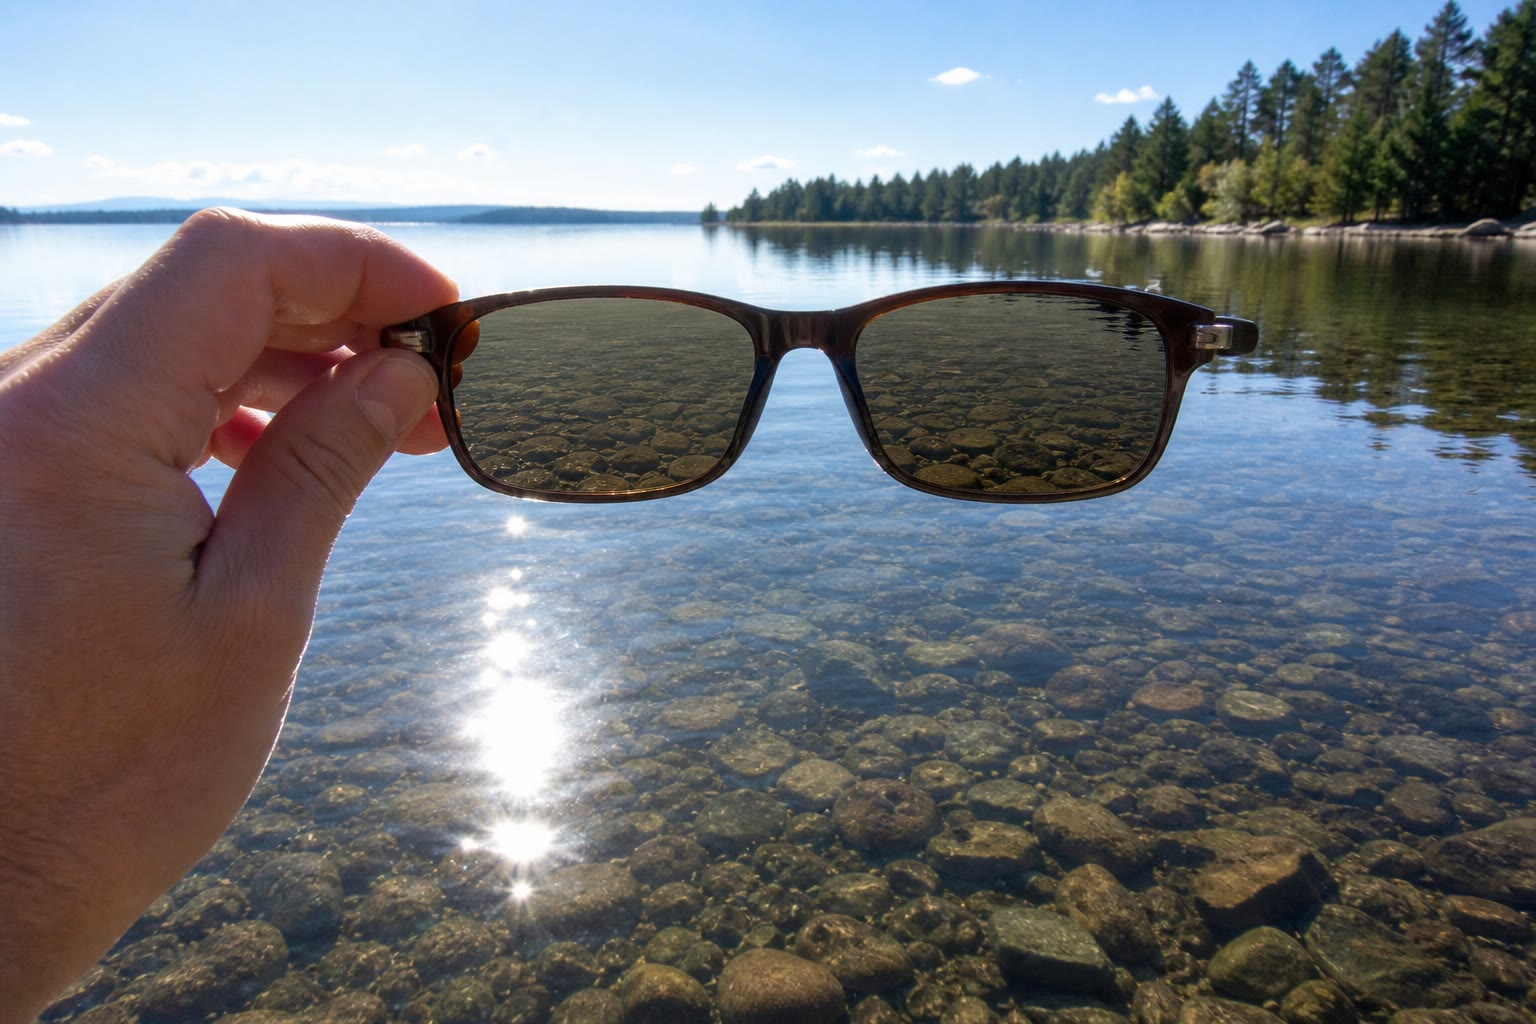
\includegraphics[width=0.58\linewidth]{images/book4/ai/b4-13-polarizing-sunglasses-lake.jpg}

{\small نظارة شمسية مستقطِبة أمام بحيرة: الوهج، المنعكس بجوار زاوية بروستر والمستقطَب أفقيًّا، يقصّه محور النفاذ الشاقولي في العدستين، فيظهر قاع البحيرة.}
\end{omfigure}

\section{مسألة: الموجة والشاشة والشراع}

\begin{problem}[{مسألة نهاية الأسبوع --- حزمة ليزر مفكَّكة إلى
مجالاتها، وشاشة ترسم بالاستقطاب، ومركبة فضائية
تُبحر على الضوء}]
\label{pb:b2:plane-waves-polarization:1}

\medskip
\noindent\textbf{الجزء I --- الحزمة.}
ليزر هليوم--نيون يبثّ \qty{10}{mW} عند \qty{632.8}{nm} في حزمة
قطرها \qty{1.0}{mm}، مستقطَبة خطيًّا على امتداد $x$، تنتقل على امتداد
$z$.
\begin{enumerate}
  \item التواتر والعدد الموجي وطاقة الفوتون؛ وعدد الفوتونات المبثوثة في
        الثانية.
  \item الشدة؛ والسعتان $E_0$ و $B_0$؛ واكتب $\vect E(z, t)$ و
        $\vect B(z, t)$.
  \item كثافة الطاقة (الوسطى) والطاقة المحتواة في \qty{1}{m} من
        الحزمة؛ وكم يبلغ طول الحزمة المبثوثة في \qty{1}{ns}، وكم
        طول موجة تحوي؟
  \item \omterm{thm:b2:poynting-vector:poynting}{متجهة بوينتنغ}: قيمتها الوسطى وتذبذبها؛ وكمية الحركة
        المحمولة في الثانية؛ والقوة على هدف أسود وعلى مرآة.
  \item قارن $E_0$ بالمجال الذي يربط الإلكترون في
        ذرة الهيدروجين (\qty{5e11}{V/m}) و $B_0$ بمجال الأرض
        (\qty{50}{\micro T}).
  \item \omterm{prop:b2:poynting-vector:wave}{ضغط الإشعاع} على مصدّ حزمة أسود، بالباسكال.
  \item وإلكترون حرّ يوضع في الحزمة: أوجد سعة تذبذب
        سرعته في المجال الكهربائي (بإهمال القوة المغناطيسية
        أولًا)؛ ونسبة القوة المغناطيسية إلى الكهربائية عليه ---
        ولماذا تكون القوة المغناطيسية مهمَلة في المادة في الضوء العادي؟
  \item اكتب مجالات الحزمة نفسها لو كانت مستقطَبة
        دائريًّا؛ وما الذي يتغير في الشدة، وفي \omterm{thm:b2:poynting-vector:poynting}{متجهة
        بوينتنغ}، وفي توقفها على الزمن؟
  \item وتمرّ الحزمة عبر مستقطِب محوره يصنع
        \qty{30}{\degree} مع $x$: أوجد الاستطاعة النافذة؛ ثم عبر ثانٍ
        متعامد مع الأول: الاستطاعة؛ ثم أدخل بينهما
        ثالثًا عند \qty{45}{\degree} عن الأول: الاستطاعة.
\end{enumerate}

\medskip
\noindent\textbf{الجزء II --- الشاشة.}
شاشة بلورات سائلة: إضاءة خلفية (\omterm{def:b2:plane-waves-polarization:states}{ضوء طبيعي})، ومستقطِب، و
الخلية، ومستقطِب متعامد. ودون توتر تدير الخلية
الاستقطاب بمقدار \qty{90}{\degree}؛ ومع التوتر لا تفعل شيئًا.
\begin{enumerate}[resume]
  \item النسبة النافذة من شدة الإضاءة الخلفية في
        الحالة المضيئة (بمستقطِبين مثاليين)؛ وفي الحالة المظلمة.
  \item ويجعل توتر وسطي الخلية تسلك سلوك مؤخِّر
        بطور $\delta$ بين محوريها، وهما عند \qty{45}{\degree} عن
        المستقطِبين (بلا إدارة): بيّن أن النفاذ
        $\sin^2(\delta/2)$ --- وهو سلّم الرمادي.
  \item ومنظورةً عبر مستقطِب مُدار إلى \qty{90}{\degree} عن مستقطِب
        خرج الشاشة، ماذا يُرى؟ وعند \qty{45}{\degree}؟
  \item \omterm{prop:b2:plane-waves-polarization:plates}{وصفيحة ربع موجية} ملصوقة على الشاشة عند \qty{45}{\degree} عن
        مستقطِبها تجعل الخرج دائريًّا: فما الفائدة لناظر
        يرتدي نظارة شمسية مستقطِبة؟
  \item والمستقطِبات المثالية كانت لتمرّر نصف الإضاءة الخلفية في
        الحالة المضيئة؛ وتمرّر الصفائح الحقيقية $85\%$ من المثالي لكل واحدة،
        وتمرّر مرشّحات ألوان البكسل ثلث الضوء:
        أوجد النسبة من استطاعة الإضاءة الخلفية التي تبلغ الناظر في الأبيض؛
        وسمِّ الموضعين اللذين يضيع فيهما معظم الضوء.
  \item والصفائح المتعامدة الحقيقية تسرّب $0.1\%$ من الضوء: أوجد نسبة تباين
        الشاشة (المضيء على المظلم) في غرفة مظلمة.
  \item و«المستقطِبات الدائرية» عند المصوّرين مستقطِب خطي
        يتبعه \omterm{prop:b2:plane-waves-polarization:plates}{صفيحة ربع موجية} عند \qty{45}{\degree}: فماذا تتلقى
        الكاميرا، ولماذا يكون ذلك أفضل لمقسّم الحزمة الحساس
        للاستقطاب في تركيزها التلقائي من الضوء
        الخطي؟
  \item ولماذا تستعمل نظارات السينما الثلاثية الأبعاد \omterm{def:b2:plane-waves-polarization:states}{استقطابًا دائريًّا} لا
        خطيًّا؟ وماذا يحدث للتداخل بين العينين
        إذا أمال الناظر رأسه \qty{20}{\degree} بنظارة خطية
        (أي الشدة المتسرّبة إلى العين الخطأ)؟
\end{enumerate}

\medskip
\noindent\textbf{الجزء III --- الشراع.}
شراع شمسي مساحته $S = \qty{1000}{m^2}$ وكتلته الكلية $m = \qty{50}{kg}$،
عاكس عكسًا تامًّا، على $D = \qty{1.0}{au} = \qty{1.5e11}{m}$ من الشمس
($I = \qty{1.36}{kW/m^2}$؛ وثقالة الشمس \qty{5.9e-3}{m/s^2} هناك).
\begin{enumerate}[resume]
  \item قوة الإشعاع حين يواجه الشراع الشمس؛ والتسارع؛
        والنسبة إلى ثقالة الشمس.
  \item ويُمال الشراع بالزاوية $\theta$ عن مواجهة الشمس: بيّن أن
        القوة ناظمية على الشراع وتتناسب مع $\cos^2\theta$
        (فالاستطاعة المعترَضة $\times\cos\theta$، وتغيّر كمية الحركة على امتداد
        الناظمة $\times\cos\theta$).
  \item وكي يحلزن الشراع خارجًا يبقي مركّبة قوة على امتداد
        سرعته المدارية: أوجد، من أجل $\theta = \qty{35}{\degree}$، التسارع
        المماسي؛ والسرعة المكتسبة في السنة؛ وقارنها بسرعة الأرض
        المدارية (\qty{30}{km/s}).
  \item ولماذا ينال الشراع نفسه، بجوار عطارد ($D = \qty{0.39}{au}$)،
        $6.6$ أضعاف القوة، ولماذا تبقى النسبة إلى الثقالة
        على حالها؟
  \item وغشاء الشراع \qty{2}{\micro m} من بلاستيك مؤلمَن: أوجد
        درجة حرارته في ضوء الشمس إذا امتصّ $10\%$ وأشعّ من
        وجهيه إشعاعَ جسم أسود ($\sigma = \qty{5.67e-8}{W.m^{-2}.K^{-4}}$).
  \item الزمن اللازم لكسب \qty{1}{km/s} في مواجهة الشمس؛ وما الذي كان
        شراع أسود (ماصّ) بالحجم نفسه ليبلغه؟
  \item تحقق من كمية حركة الضوء بالفوتونات: أوجد عدد الفوتونات
        التي تصيب الشراع في الثانية (بمتوسط \qty{2}{eV}) و
        كمية حركة كل منها $hf/c$؛ ثم استعد القوة.
  \item لخّص: المقادير الثلاثة التي تحملها الموجة (الطاقة، و
        كمية الحركة، والاستقطاب) والجهاز في هذه المسألة الذي
        يستثمر كلًّا منها.
\end{enumerate}
\end{problem}
